This package provides functions to analyze sets of objects in 2D and 3D. It provides the computation of axis-aligned bounding boxes, centers of mass and principal component analysis for all bounded objects, as well as barycenters for sets of weighted points. Note that unlike most of the CGAL packages, this package uses approximation methods (in particular for linear least squares fitting) and is not intended to provide an exact canonical result in any sense. 

\section{Definitions}

A \emph{bounding box} for a set of objects is a cuboid that contains the set. An \emph{axis-aligned bounding box} is a an expression of the maximum extents of all objects from the set within their coordinate system, i.e., a bounding box aligned with the axes of the coordinate system. Axis-aligned bounding boxes are frequently used in geometric algorithms as an indication of the general position of a data set, for either display, first-approximation spatial query, or spatial indexing purposes. \\

A \emph{centroid} of a set of objects is their center of mass, i.e., the point whose coordinates are computed by means of coordinates of all points composing the objects. Note that although the general definition of center of mass incorporates a density function (and hence weighted means), the current implementation assumes a uniform density (see barycenter below defined for weighted points). For a point set $\{X_1,X_2,...,X_N\}$ the centroid $\bar{X}$ is computed as $$\bar{X} = \frac{1}{N} \ccSum{i=1}{N}{ X_i}.$$ For a set of segments $\{S_1,S_2,...,S_N\}$ the centroid $\bar{X}$ is computed as $$\bar{X} = \frac{1}{\ccSum{i=1}{N}{\left|S_i\right|}} \ccSum{i=1}{N}{ \left|S_i\right| \bar{S_i}},$$ where $\left|S_i\right|$ stands for the length of a segment and $\bar{S_i}$ stands for its uniform barycenter (midpoint). For a set of triangles $\{T_1,T_2,...,T_N\}$ the centroid $\bar{X}$ is computed as $$\bar{X} = \frac{1}{\ccSum{i=1}{N}{\left|T_i\right|}} \ccSum{i=1}{N}{ \left|T_i\right| \bar{T_i}},$$ where $\left|T_i\right|$ stands for the area of a triangle and $\bar{T_i}$ stands for its uniform barycenter. Such definition still holds for more general objects where the Lebesgue measure (length in 1D, area in 2D, volume in 3D) is used for weighting the object barycenters. Centers of mass are used to summarize data sets for either approximation, spatial query or spatial indexing purposes.\\

A \emph{barycenter} of a set of weighted points is the point whose coordinates are computed by means of weighted coordinates of all weighted points from the set. When all weights are equal the barycenter coincides with the centroid.\\

Given a set of objects, \emph{linear least squares fitting} amounts to finding the linear sub-space which minimizes the sum of squared distances from all points composing the objects of the set, to their projection onto this linear sub-space. Such linear sub-space is obtained by so-called principal component analysis (PCA). PCA is defined as a transformation that transforms the objects to a new coordinate system such that the greatest variance by orthogonal projection of the objects comes to lie on the first coordinate (called the first principal component), the second greatest variance on the second coordinate, and so on. PCA is often used in geometric applications to reduce data sets to lower dimensions for analysis or approximation. Figure below illustrates (least squares) fitting of a line to a 2D point set, fitting of a line and a plane to a 3D point set and fitting of a plane to a set of 3D triangles. 

\begin{center}
    \label{fit}
    % Image
    \begin{ccTexOnly}
      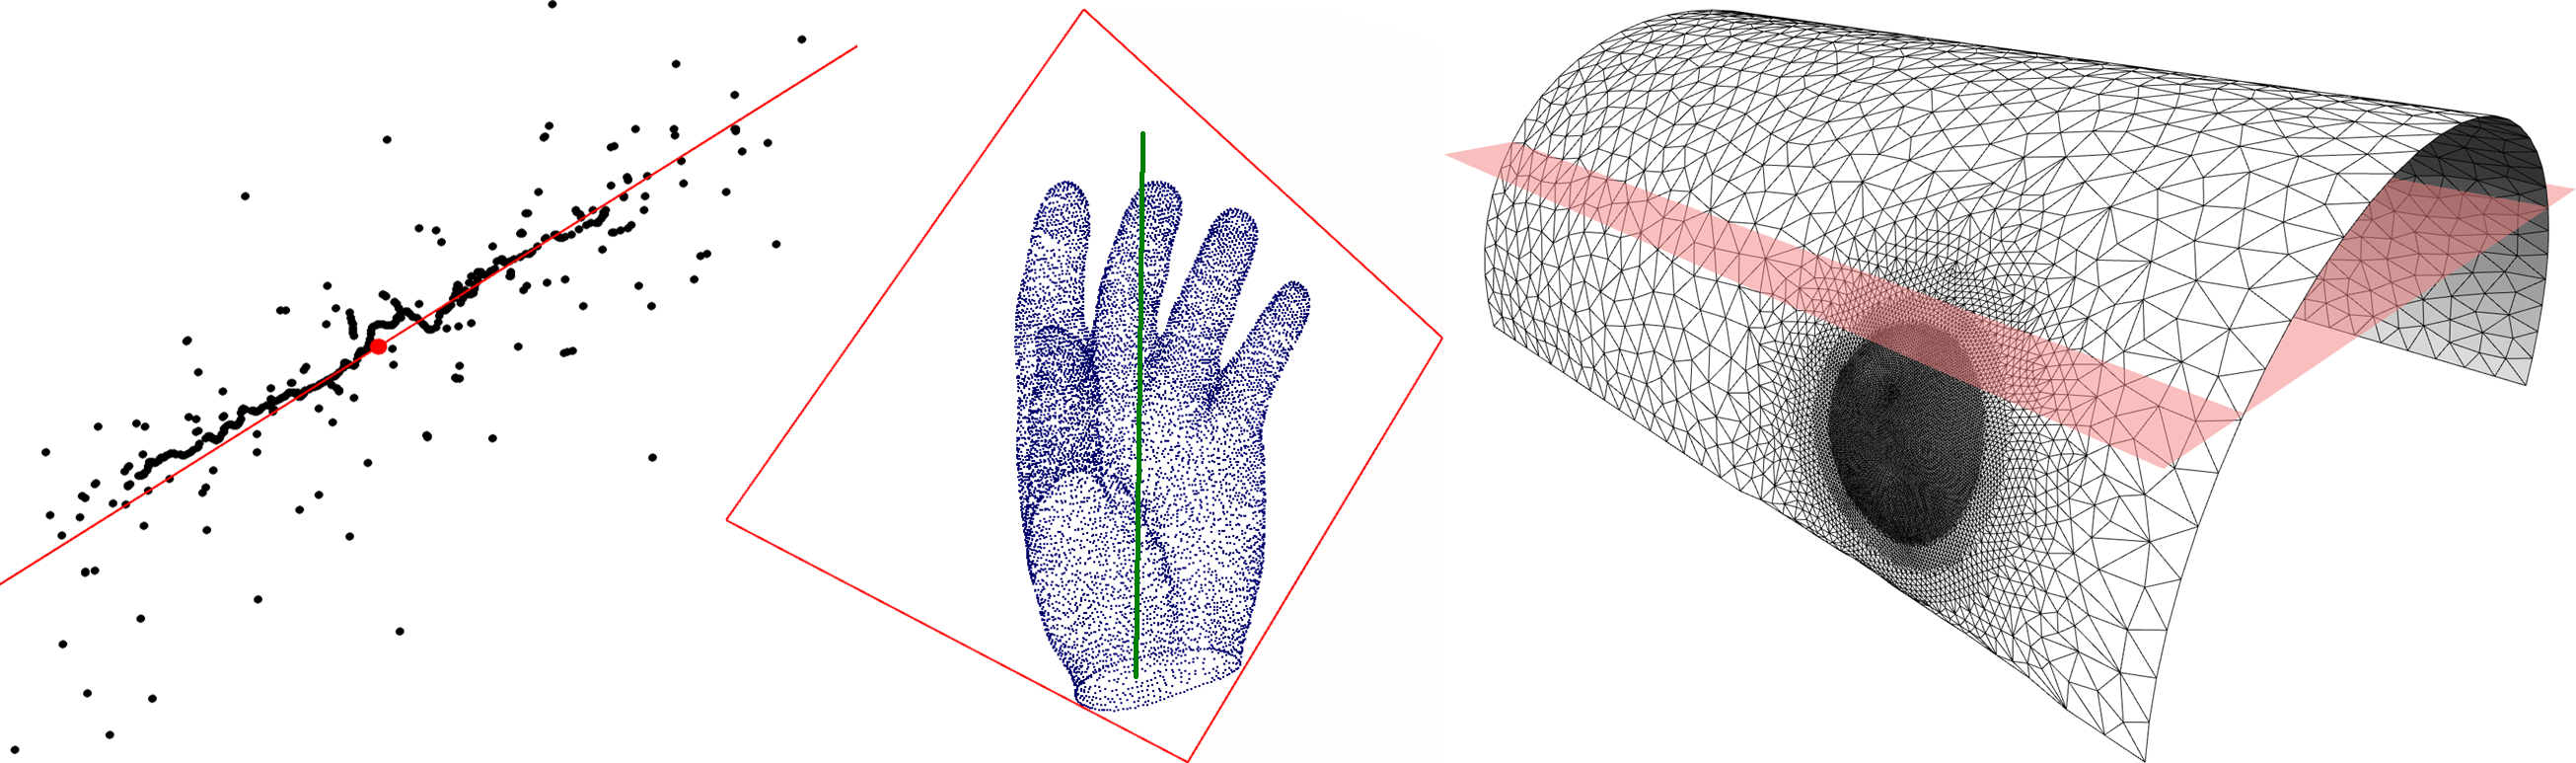
\includegraphics[width=1.0\textwidth]{Principal_component_analysis/fit}
    \end{ccTexOnly}
    \begin{ccHtmlOnly}
        <img width="100%" border=0 src="./fit.png"><P>
    \end{ccHtmlOnly}
    % Title
    \begin{figure}[h]
        \caption{Left: fitting a line to a 2D point set (centroid dotted in red).
                 Middle: fitting a line and a plane to a 3D point set.
                 Right: fitting a plane to a set of 3D triangles.}
    \end{figure}
\end{center}

